% Provenance (never printed): see sources/outline_sources.md (Year 3:
% geomorphology, hillslope processes, river incision, landscape evolution).
% Brief: sources/book5/BRIEFS.md, ch. 18. Curves from
% figdata/bachelor-3/hillslope.py, stream_profile.py and varden_river.py.
% Exercise and problem values in the Book 5 scratch calculator calc/ch18.py.
% The upland west of the Varden Hills, its river, its tributaries, its
% uplift rate and its base-level fall are invented; the outlet elevation is
% the region model's river at the west edge of the map.
\chapter{Kwantitatieve geomorfologie}\label{ch:b3:quantitative-geomorphology}

Een rivier die een opkomend gebergte kruist heeft een stap in zijn lengteprofiel: een waterval,
met daaronder een ravijn en erboven een zachtere vallei. De stap blijft niet
waar hij ontstond. Hij klimt stroomopwaarts, enkele millimeters of enkele meters per
jaar, en zijn positie is een klok die begon te lopen toen het \omterm{def:b3:quantitative-geomorphology:knickpoint}{basisniveau} van de rivier
werd verlaagd. Die klok aflezen, en de snelheden die in de vormen van heuvels en rivieren zijn vastgelegd,
vraagt om twee behoudswetten en twee transportwetten: één voor de grond die langs een helling kruipt,
en één voor het vaste gesteente dat een rivier uitsnijdt.

\begin{recall}
Verwering, erosie, afzetting, reliëfvormen en het evenwicht tussen opheffing
en erosie staan in de schoolboeken, net als isostatisch herstel en U-vormige
gletsjerdalen. De denudatiesnelheid, de bodemschuifspanning en de
Shields-parameter staan in Boek~3, in het hoofdstuk over erosie en transport;
het digitaal hoogtemodel in het hoofdstuk over geologische kaarten; de
Airy-isostasie in het hoofdstuk over isostasie en zwaartekrachtsanomalieën. Kosmogene
nucliden en daaruit afgeleide erosiesnelheden staan in
Hoofdstuk~\ref{ch:b3:advanced-geochronology}, \omterm{def:b3:orogenic-wedges:thermochronology}{thermochronologie} en de
\omterm{def:b3:orogenic-wedges:age-elevation}{ouderdom--hoogterelatie} staat in Hoofdstuk~\ref{ch:b3:orogenic-wedges}. De
diffusievergelijking staat in de natuurkundeboeken.
\end{recall}

\section{Hellingen}\label{sec:b3:quantitative-geomorphology:hillslopes}

Op een heuvel met een bodemlaag beweegt de grond korrel voor korrel naar beneden: graafdieren
gooien hem rond, wortels tillen hem op, vriezen en bevochtigen doen hem zwellen, en elke
verstoring laat de zwaartekracht hem een beetje verschuiven. Over eeuwen gemiddeld is de
bodemflux evenredig met de helling.

\begin{definition}[Hellingdiffusie]\label{def:b3:quantitative-geomorphology:diffusion}
\emph{Hellingdiffusie}\index{hellingdiffusie} is het langzame
transport van grond naar beneden waarvan de volumeflux per eenheid van breedte van de helling,
$\vec q$, is evenredig met de gradiënt van de oppervlaktehoogte $z$:
$\vec q = -\kappa\,\nabla z$. De coëfficiënt $\kappa$, in
\unit{m^2/yr}, is de hellingdiffusiviteit.
\end{definition}

\begin{theorem}[Diffusie van hellingen]\label{thm:b3:quantitative-geomorphology:diffusion}
Stel dat het gesteente met snelheid $U$ wordt opgeheven ten opzichte van de geulen die een
helling begrenzen, dat grond en gesteente dezelfde dichtheid hebben en dat grond zich door \omterm{def:b3:quantitative-geomorphology:diffusion}{hellingdiffusie}
verplaatst met uniforme $\kappa$. Dan voldoet de oppervlaktehoogte aan
\[
\frac{\partial z}{\partial t} = U + \kappa\,\nabla^2 z ,
\]
de diffusievergelijking met een bronterm.
\end{theorem}

\begin{proof}
Neem een klein gebied $\delta S$ van de helling. Het volume ervan verandert door opheffing,
$U\,\delta S$ per tijdseenheid, en door de grond die via zijn
randen naar buiten stroomt, $\oint \vec q\cdot\vec n\,\mathrm{d}\ell = (\nabla\cdot\vec q)\,\delta S$.
Hieruit volgt $\partial z/\partial t = U - \nabla\cdot\vec q$; met $\vec q = -\kappa
\nabla z$ en $\kappa$ uniform, geldt $\nabla\cdot\vec q = -\kappa\nabla^2 z$.
\end{proof}

Een breuk of een kustlijn snijdt op één moment een steilrand uit; daarna
verandert de steilrand alleen nog door diffusie. Uitgaande van een verticale stap met halve hoogte $a$ op een verre
helling $b$ is de oplossing in één dimensie:
\[
z(x,t) = a\,\operatorname{erf}\!\left(\frac{x}{2\sqrt{\kappa t}}\right) + b\,x ,
\qquad
\left.\frac{\partial z}{\partial x}\right|_{x=0} = \frac{a}{\sqrt{\pi\kappa t}} + b .
\]
De vorm hangt alleen af van het product $\kappa t$: een gemeten profiel geeft
$\kappa t$, en ofwel levert een onafhankelijke ouderdom $\kappa$, ofwel levert een bekende
$\kappa$ levert de ouderdom, een \emph{morfologische ouderdom}. Steilranden in semi-aride
gebieden met korrelige bodems en schaarse begroeiing geven $\kappa$ tussen
$10^{-3}$ en \qty{e-2}{m^2/yr}; vochtige, dicht begroeide kustgebergten
ongeveer \qty{5e-3}{m^2/yr}.
% ledger: whipple04:scarp-erf, whipple04:scarp-kappa

\begin{omfigure}
\begin{tikzpicture}
\begin{groupplot}[group style={group size=2 by 1, horizontal sep=1.6cm},
  width=0.48\linewidth, height=0.36\linewidth, tick label style={font=\scriptsize},
  label style={font=\small}, legend style={font=\scriptsize, draw=none, fill=none}]
\nextgroupplot[xlabel={afstand $x$ (m)}, ylabel={$z$ (m)}, xmin=-40, xmax=40,
  ymin=-5, ymax=5, legend pos=north west]
% computed in figdata/bachelor-3/hillslope.py
\addplot[black!50, densely dashed] table[x=x, y=z0] {figdata/out/bachelor-3-hillslope-scarp.dat};
\addplot[omDef, thick] table[x=x, y=z1] {figdata/out/bachelor-3-hillslope-scarp.dat};
\addplot[omProp, thick] table[x=x, y=z2] {figdata/out/bachelor-3-hillslope-scarp.dat};
\addplot[omThm, thick] table[x=x, y=z3] {figdata/out/bachelor-3-hillslope-scarp.dat};
\legend{begin, \qty{2}{kyr}, \qty{10}{kyr}, \qty{40}{kyr}}
\nextgroupplot[xlabel={afstand tot de waterscheiding (m)}, ylabel={hoogte (m)},
  xmin=-150, xmax=150, ymin=0, ymax=200, xtick={-150,-75,0,75,150}]
\addplot[omMeth, thick] table[x=x, y=z1] {figdata/out/bachelor-3-hillslope-hill.dat};
\addplot[omDef, thick] table[x=x, y=z2] {figdata/out/bachelor-3-hillslope-hill.dat};
\addplot[omThm, thick] table[x=x, y=z3] {figdata/out/bachelor-3-hillslope-hill.dat};
\node[font=\scriptsize, anchor=north] at (axis cs:0,45) {0.0215};
\node[font=\scriptsize, anchor=north] at (axis cs:0,94) {0.043};
\node[font=\scriptsize, anchor=north] at (axis cs:0,184) {\qty{0.086}{mm/yr}};
\end{groupplot}
\end{tikzpicture}

\par\smallskip{\small Links, een steilrand met een verval van \qty{5}{m} op een helling van
0.05, die diffundeert met $\kappa = \qty{5e-3}{m^2/yr}$: de beginstap
(gestippeld) en de profielen na 2, 10 en \qty{40}{kyr}. Rechts, stationaire
heuvels met een halve breedte van \qty{150}{m} en dezelfde $\kappa$ (hoogte boven de
geulen), die dalen met
0.0215, 0.043 en \qty{0.086}{mm/yr}: parabolen waarvan het reliëf en de kromming op de top
evenredig zijn met de erosiesnelheid.}\label{fig:b3:quantitative-geomorphology:hillslope}
\end{omfigure}
% ledger: whipple04:scarp-kappa

Wanneer een heuvel lang genoeg is opgeheven en geërodeerd, verandert
zijn vorm niet meer: elk punt daalt met de snelheid waarmee de rots omhoog komt.

\begin{proposition}[Kromming van de top bepaalt de erosiesnelheid]\label{prop:b3:quantitative-geomorphology:curvature}
Op een helling in \omterm{def:b3:quantitative-geomorphology:steady-profile}{stationaire toestand} onder \omterm{def:b3:quantitative-geomorphology:diffusion}{hellingdiffusie} wordt de erosiesnelheid
$E$, gelijk aan $U$, gegeven door
\[
E = -\kappa\,\nabla^2 z .
\]
In één dimensie is het profiel de parabool $z = z_0 - E x^2/(2\kappa)$,
met reliëf $E L^2/(2\kappa)$ tussen de waterscheiding en de geulen op een afstand
$L$ verwijderd.
\end{proposition}

\begin{proof}
Door $\partial z/\partial t = 0$ in de stelling te stellen, volgt $\kappa\nabla^2 z =
-U = -E$. In één dimensie geven twee integraties, met $\mathrm{d}z/\mathrm{d}x =
0$ aan de waterscheiding de parabool, en de waarde ervan bij $x = L$ het reliëf.
\end{proof}

Kromming, een geometrische grootheid die op een digitaal hoogtemodel wordt gemeten, leest zo
als snelheid zodra $\kappa$ bekend is: hoe steiler en scherper afgerond de
heuveltoppen, hoe sneller het landschap erodeert. De bodem zelf ontstaat uit
de onderliggende rots met een snelheid die afhangt van hoeveel bodem er al op ligt.

\begin{definition}[Bodemproductiefunctie]\label{def:b3:quantitative-geomorphology:soil-production}
De \emph{bodemproductiefunctie}\index{bodemproductiefunctie} geeft
de snelheid $P$ waarmee vaste gesteente wordt omgezet in bodem als functie van de
bodemdikte $h$; zij wordt meestal genomen als $P = P_0\,e^{-h/h_0}$, waarbij
$P_0$ de snelheid op kaal gesteente is en $h_0$ een lengte van enkele decimeters.
\end{definition}

In \omterm{def:b3:quantitative-geomorphology:steady-profile}{stationaire toestand} daalt het grensvlak tussen bodem en rots met de snelheid van het
oppervlak, $P(h) = E$, zodat de bodemdikte $h = h_0 \ln(P_0/E)$ is: snellere erosie betekent
dunnere bodem, en waar $E$ groter is dan $P_0$ is de bodem
weggeslagen en komt kaal gesteente, beperkt door verwering, aan de oppervlakte. De snelste
gemeten bodemproductiesnelheden bedragen de orde van \qty{0.5}{mm/yr}.
% ledger: whipple04:soil

Lineaire diffusie faalt op steile hellingen. Naarmate de gradiënt een
drempelwaarde nadert, rollen en glijden korrels in stoten en ontdoen ondiepe
aardverschuivingen de bodem van haar bedekking.

\begin{definition}[Kritische hellinggradiënt]\label{def:b3:quantitative-geomorphology:critical}
De \emph{kritische hellinggradiënt}\index{kritische hellinggradiënt}
$S_c$ is de gradiënt waarbij de bodemflux onbeperkt groeit; in een
veelgebruikte niet-lineaire transportwet geldt $q = \kappa S/[1 - (S/S_c)^2]$.
\end{definition}

Hellingen die veel flauwer zijn dan $S_c$ gedragen zich als bij lineaire diffusie; hellingen die
snel eroderen worden steiler richting $S_c$ en worden vlak, hun gradiënt wordt bepaald door de
drempelwaarde en niet door de erosiesnelheid.
% ledger: whipple04:nonlinear

\begin{inthefield}[Een hellingprofiel inmeten]
Een team dat een met bodem bedekte rug in kaart brengt, zet een terrestrische laserscanner op een
statief op enkele tientallen meters van de kam. Elke scan registreert miljoenen
punten, de afstand en richting tot het grondoppervlak, door openingen in
het gras en de struiken heen; de punten van meerdere scanstations worden samengevoegd
tot één puntenwolk, ingepast op doelen die met een satellietontvanger zijn ingemeten,
en de laatste reflecties worden bewaard om de vegetatie te verwijderen. De kale-bodemwolk
wordt omgezet in een hoogtemodel met cellen van een decimeter, gladgestreken over enkele
meters, en de Laplaciaan ervan wordt op de kam berekend. Het team vergelijkt vervolgens de
topkrommingen van ruggen die eroderen met snelheden gemeten met kosmogene
nucliden: uitgezet tegen elkaar geven de twee de diffusiviteit van de
helling als de helling van een lijn, zoals de propositie voorspelt.
\end{inthefield}

\section{Riviererosie}\label{sec:b3:quantitative-geomorphology:rivers}

Waar een rivier over vaste gesteente stroomt, snijdt zij zich omlaag door blokken los te trekken,
door schuring onder haar bedlast en door cavitatie. Al deze processen schalen met de schuifspanning
die de stroming op haar bodem uitoefent, of met het vermogen dat zij daar verbruikt, en beide nemen toe
met afvoer en helling. De afvoer neemt toe met het afwateringsgebied, dus staat
het afwateringsgebied voor de afvoer.

\begin{definition}[Stroomvermogenswet]\label{def:b3:quantitative-geomorphology:stream-power}
De \emph{stroomvermogenswet}\index{stroomvermogenswet} geeft de snelheid van
verticale insnijding $E$ van een rivier op vast gesteente als
\[
E = K A^m S^n ,
\]
waarbij $A$ het afwateringsgebied stroomopwaarts van het punt is, $S$ de helling van de
geul, $m$ en $n$ positieve exponenten, en $K$ een erodeerbaarheidscoëfficiënt
die gesteentesterkte, klimaat en geulbreedte samenvat.
\end{definition}

Voor processen die schalen met de schuifspanning of met het eenheidsstroomvermogen
ligt $m/n$ dicht bij 0.5. Een onderzoek naar badlandgeulen die in zwakke rots
zijn uitgesneden gedurende ongeveer 20 jaar, vond insnijdingssnelheden evenredig met $A^{0.44}S^{0.68}$.
% ledger: whipple04:spim

\begin{definition}[Losmakingsbeperkte en transportbeperkte insnijding]\label{def:b3:quantitative-geomorphology:limited}
Insnijding is \emph{losmakingsbeperkt}\index{losmakingsbeperkte insnijding}
wanneer de rivier meer sediment kan afvoeren dan zij ontvangt, zodat haar
daalsnelheid wordt bepaald door hoe snel zij vaste gesteente van haar bodem losmaakt: de
\omterm{def:b3:quantitative-geomorphology:stream-power}{stroomvermogenswet} geldt dan. Zij is
\emph{transportbeperkt}\index{transportbeperkte insnijding} wanneer de rivier al het
sediment vervoert dat zij kan dragen, zodat haar bodem alleen daalt waar de
transportcapaciteit stroomafwaarts toeneemt, met een snelheid die wordt bepaald door
de divergentie van de sedimentflux.
\end{definition}

Een \omterm{def:b3:quantitative-geomorphology:limited}{transportbeperkte} rivier gedraagt zich in grote lijnen als een helling: de flux hangt
af van de helling, en haar profiel evolueert via een diffusieachtige vergelijking die
elke trede afrondt. Een \omterm{def:b3:quantitative-geomorphology:limited}{losmakingsbeperkte} rivier houdt een trede scherp en verplaatst die,
zoals de volgende paragraaf laat zien. Bergrivieren met vaste gesteentebodems en dun
grind liggen meestal dichter bij het eerste type; rivieren op dik alluvium bij het
tweede.

\begin{omfigure}
\begin{tikzpicture}[x=0.55cm, y=0.55cm, font=\scriptsize,
  declare function={f(\x)=2.1+3.5*(1-(\x-0.5)/10)^2;
    tl(\x,\l)=f(\x)-1.1*exp(-(10.5-\x)/\l);}]
\begin{scope}
\draw[->] (0,0) -- (11.5,0) node[below left] {afstand stroomafwaarts};
\draw[->] (0,0) -- (0,6) node[above right] {$z$};
\draw[black!50, densely dashed] plot[domain=0.5:10.5, samples=40] (\x,{f(\x)});
\draw[omDef, thick] plot[domain=0.5:6.5, samples=30] (\x,{f(\x)}) -- plot[domain=6.5:10.5, samples=20] (\x,{f(\x)-1.1});
\draw[omThm, thick] plot[domain=0.5:3.5, samples=20] (\x,{f(\x)}) -- plot[domain=3.5:10.5, samples=30] (\x,{f(\x)-1.1});
\draw[->, black!70] (6.3,4.1) -- (3.8,4.75);
\node[anchor=west, align=left] at (5.6,5.3) {losmakingsbeperkt:\\ de trap schuift stroomopwaarts};
\node at (5.5,-0.7) {(a)};
\end{scope}
\begin{scope}[xshift=7.2cm]
\draw[->] (0,0) -- (11.5,0) node[below left] {afstand stroomafwaarts};
\draw[->] (0,0) -- (0,6) node[above right] {$z$};
\draw[black!50, densely dashed] plot[domain=0.5:10.5, samples=40] (\x,{f(\x)});
\draw[omDef, thick] plot[domain=0.5:10.5, samples=40] (\x,{tl(\x,1.2)});
\draw[omThm, thick] plot[domain=0.5:10.5, samples=40] (\x,{tl(\x,3.5)});
\node[anchor=west, align=left] at (5.0,5.3) {transportbeperkt:\\ de val diffundeert stroomopwaarts};
\node at (5.5,-0.7) {(b)};
\end{scope}
\end{tikzpicture}

\par\smallskip{\small De respons van een rivier op een daling van haar \omterm{def:b3:quantitative-geomorphology:knickpoint}{basisniveau}
(gestippeld: het profiel vóór de daling; blauw, daarna rood: twee latere tijden),
schematisch. (a) Een \omterm{def:b3:quantitative-geomorphology:limited}{losmakingsbeperkte} rivier behoudt een scherp \omterm{def:b3:quantitative-geomorphology:knickpoint}{knikpunt} dat
stroomopwaarts migreert; daaronder heeft het profiel zijn oude vorm, maar lager. (b) Een
\omterm{def:b3:quantitative-geomorphology:limited}{transportbeperkte} rivier verlaagt haar hele profiel geleidelijk, het sterkst
nabij de monding.}\label{fig:b3:quantitative-geomorphology:regimes}
\end{omfigure}

Als gesteente met een uniforme snelheid $U$ ten opzichte van de monding van de rivier stijgt, en $K$,
$m$, $n$ uniform zijn, evolueert de rivier volgens $\partial z/\partial t = U - K A^m
S^n$.

\begin{definition}[Stationair rivierprofiel]\label{def:b3:quantitative-geomorphology:steady-profile}
Een rivierprofiel bevindt zich in een \emph{stationaire toestand}\index{stationair rivierprofiel}
wanneer zijn hoogte niet langer in de tijd verandert: op elk punt compenseert
insnijding precies de opheffing van het gesteente ten opzichte van de monding.
\end{definition}

\begin{theorem}[Stationair profiel onder de stroomvermogenswet]\label{thm:b3:quantitative-geomorphology:steady}
Bij uniforme $U$, $K$, $m$ en $n$ heeft een \omterm{def:b3:quantitative-geomorphology:limited}{losmakingsbeperkte} rivier in \omterm{def:b3:quantitative-geomorphology:steady-profile}{stationaire
toestand} de hellinggradiënt
\[
S = \left(\frac{U}{K}\right)^{1/n} A^{-m/n} .
\]
\end{theorem}

\begin{proof}
In de \omterm{def:b3:quantitative-geomorphology:steady-profile}{stationaire toestand} geldt $\partial z/\partial t = 0$, dus $K A^m S^n = U$, waaruit $S^n
= (U/K)A^{-m}$ volgt; het nemen van de $n$-de wortel geeft het resultaat.
\end{proof}

\begin{omfigure}
\begin{tikzpicture}
\begin{groupplot}[group style={group size=2 by 1, horizontal sep=1.7cm},
  width=0.48\linewidth, height=0.33\linewidth, tick label style={font=\scriptsize},
  label style={font=\small}]
\nextgroupplot[xlabel={afstand van de waterscheiding (km)}, ylabel={$z$ (m)},
  xmin=0, xmax=12, ymin=150, ymax=420]
% computed in figdata/bachelor-3/stream_profile.py
\addplot[omDef, thick] table[x=d, y=z] {figdata/out/bachelor-3-stream_profile-steady.dat};
\nextgroupplot[xmode=log, ymode=log, xlabel={afwateringsgebied $A$ (\unit{km^2})},
  ylabel={gradiënt $S$}, xmin=0.1, xmax=100, ymin=0.003, ymax=0.2]
\addplot[omDef, thick] table[x=A, y=S] {figdata/out/bachelor-3-stream_profile-steady.dat};
\addplot[only marks, mark=*, mark size=1.4pt, omThm] table[x=A, y=S] {figdata/out/bachelor-3-stream_profile-sa.dat};
\addplot[omThm, densely dashed] table[x=A, y=S] {figdata/out/bachelor-3-stream_profile-fit.dat};
\end{groupplot}
\end{tikzpicture}

\par\smallskip{\small Het stationaire profiel van de verzonnen heuvelrivier
ten westen van de Varden Hills ($U = \qty{0.043}{mm/yr}$, $K =
\qty{e-6}{yr^{-1}}$, $m = 0.5$, $n = 1$), van het bronpunt tot de
monding op \qty{170}{m}. Rechts: gradiënt tegen oppervlakte: het model (blauwe
lijn) en twaalf gradiënten gemeten over trajecten van \qty{200}{m} met een
spreiding van ongeveer \qty{10}{\percent} (rode stippen), waarvan de kleinste-kwadratenlijn
(gestippeld) een helling van $-0.47$ heeft.}\label{fig:b3:quantitative-geomorphology:profile}
\end{omfigure}

Het verloop van de gradiënt volgt een machtsverband met de oppervlakte: het profiel is
concaaf omhoog. Echte rivieren volgen zo'n machtswet ook als de veronderstellingen van de stelling
twijfelachtig zijn, zodat twee getallen een profiel samenvatten.
% ledger: whipple04:steepness

\begin{definition}[Steilheids- en concaviteitsindices van de geul]\label{def:b3:quantitative-geomorphology:indices}
Volgt de gradiënt van een rivier $S = k_s A^{-\theta}$, dan is de exponent
$\theta$ de \emph{concaviteitsindex}\index{concaviteitsindex} en de
coëfficiënt $k_s$ de \emph{geulsteilheidsindex}\index{geulsteilheidsindex}.
Om rivieren te vergelijken wordt $\theta$ gelijkgesteld aan een gemeenschappelijke referentiewaarde
$\theta_{\mathrm{ref}}$, en $k_{sn} = S A^{\theta_{\mathrm{ref}}}$ is de
genormaliseerde steilheid.
\end{definition}

Volgens de stelling geldt $\theta = m/n$ en $k_s = (U/K)^{1/n}$: bij een gegeven
erodeerbaarheid is een rivier steiler waar het gesteente sneller stijgt. Steilheidskaarten van een
gebergte geven daarom de opheffing weer.


Gradiënten zijn afgeleiden van ruisrijke hoogtes en lopen sterk uiteen. Het integreren
van het profiel gebruikt daarentegen hoogtes, die beter te meten zijn.

\begin{definition}[Chi-analyse]\label{def:b3:quantitative-geomorphology:chi}
\emph{Chi-analyse}\index{chi-analyse} zet de hoogte van de punten
van een riviernetwerk uit tegen de coördinaat
\[
\chi(x) = \int_{x_b}^{x} \left(\frac{A_0}{A(x')}\right)^{\theta}
\mathrm{d}x' ,
\]
waarbij $x$ de afstand stroomopwaarts langs de geul vanaf een basispunt
$x_b$ is, $A_0$ een referentieoppervlakte en $\theta$ de \omterm{def:b3:quantitative-geomorphology:indices}{concaviteitsindex}; $\chi$ heeft
de dimensie van een lengte.
\end{definition}

\begin{proposition}[De chi-transformatie maakt een stationair profiel recht]\label{prop:b3:quantitative-geomorphology:chi}
Onder de aannames van de stationaire-toestandsstelling, met $\theta = m/n$,
voldoet elke geul van een netwerk dat afwatert naar het \omterm{def:b3:quantitative-geomorphology:knickpoint}{basisniveau} $z_b$ aan
\[
z = z_b + \left(\frac{U}{K A_0^{m}}\right)^{1/n} \chi :
\]
alle geulen liggen op één rechte lijn met helling $k_s A_0^{-\theta}$ in het
$(\chi, z)$-vlak.
\end{proposition}

\begin{proof}
Langs een geul geldt $\mathrm{d}z/\mathrm{d}x = S = k_s A^{-\theta} = k_s
A_0^{-\theta}(A_0/A)^{\theta}$. Integratie vanaf $x_b$, waar $z = z_b$,
geeft $z = z_b + k_s A_0^{-\theta}\chi$, en $k_s A_0^{-\theta} =
(U/K)^{1/n} A_0^{-m/n}$. Een zijrivier sluit aan op de hoofdrivier in een splitsingspunt waarvan
$z$ en $\chi$ deelt, en voldoet stroomopwaarts daarvan aan dezelfde relatie.
\end{proof}

Een geul die van de lijn afwijkt, is niet in \omterm{def:b3:quantitative-geomorphology:steady-profile}{stationaire toestand}, of snijdt
gesteente met een andere erodeerbaarheid, of heeft afwateringsgebied verloren of
verworven: een zijrivier die bij dezelfde $\chi$ boven haar buren ligt, wordt
van oppervlakte beroofd, en een die lager ligt, groeit.

\section{Transiënte landschappen}\label{sec:b3:quantitative-geomorphology:transient}

\begin{definition}[Basisniveau en knikpunt]\label{def:b3:quantitative-geomorphology:knickpoint}
Het \emph{basisniveau}\index{basisniveau} van een rivier is de hoogte van haar
monding, waaronder zij niet kan insnijden: de zee, een meer, of de hoofdrivier
waarin zij uitmondt. Een \emph{knikpunt}\index{knikpunt} is een plaats waar de
helling van het lengteprofiel van een rivier abrupt toeneemt, van een steiler
geworden traject tot een waterval.
\end{definition}

Een \omterm{def:b3:quantitative-geomorphology:knickpoint}{knikpunt} kan vast zijn, waar de rivier een harder bed kruist of een
breukwand die nog actief is, of mobiel zijn, waar het de kop vormt van de
reactie van de rivier op een verandering stroomafwaarts: een daling van het \omterm{def:b3:quantitative-geomorphology:knickpoint}{basisniveau}, een
snellere opheffing.
% ledger: whipple04:response

\begin{theorem}[Knikpunten als kinematische golven]\label{thm:b3:quantitative-geomorphology:kinematic}
Neem $n = 1$, met $U$, $K$ en $m$ uniform, en laat $x$ de afstand stroomopwaarts
vanaf de monding zijn. Dan voldoet $z$ aan
\[
\frac{\partial z}{\partial t} + K A^m \frac{\partial z}{\partial x} = U ,
\]
en elk kenmerk van het profiel, ook een stap, beweegt stroomopwaarts met de
snelheid $c = K A^m$ en behoudt daarbij zijn hoogte. Een \omterm{def:b3:quantitative-geomorphology:knickpoint}{knikpunt} dat aan de
monding begint op $t = 0$ bereikt het punt $x$ op het tijdstip
\[
t(x) = \int_0^x \frac{\mathrm{d}x'}{K A(x')^m} = \frac{\chi(x)}{K A_0^m},
\]
met $\chi$ berekend met $\theta = m$. Alle \omterm{def:b3:quantitative-geomorphology:knickpoint}{knikpunten} die in een netwerk tegelijk
ontstaan, liggen dus bij dezelfde $\chi$ en op dezelfde hoogtelijn.
\end{theorem}

\begin{proof}
Met $x$ stroomopwaarts is de helling $S = \partial z/\partial x$, en de
evolutievergelijking $\partial z/\partial t = U - K A^m S$ is de vergelijking
zoals hierboven geschreven. Langs een kromme $\mathrm{d}x/\mathrm{d}t = K A(x)^m$,
is het linkerlid de totale afgeleide $\mathrm{d}z/\mathrm{d}t$, dus $z$ stijgt met $U$ per
tijdseenheid langs elke zodanige kromme. Twee punten aan weerszijden van een stap,
die langs naburige krommen meebewegen, krijgen dezelfde hoogte erbij, dus de stap
behoudt zijn hoogte en beweegt mee met de krommen. De tijd om $x$ te bereiken is
$\int \mathrm{d}x'/c$, wat $\chi(x)/(K A_0^m)$ is volgens de definitie van
$\chi$ met $\theta = m$. In het netwerk wordt $\chi$ gemeten langs elk
stroompad vanaf dezelfde monding, dus gelijke tijden betekenen gelijke $\chi$, en
volgens de propositie over $\chi$ zetten de trajecten onder de \omterm{def:b3:quantitative-geomorphology:knickpoint}{knikpunten}, die
al aan het nieuwe \omterm{def:b3:quantitative-geomorphology:knickpoint}{basisniveau} zijn aangepast, ze alle op dezelfde hoogte.
\end{proof}

De snelheid van de golf neemt toe met het afwateringsgebied: een \omterm{def:b3:quantitative-geomorphology:knickpoint}{knikpunt} loopt
snel door de hoofdrivier en vertraagt in de bovenlopen. De tijd die het kost om het hele
netwerk tot aan de geulkoppen te doorlopen, is de \emph{responstijd} van het landschap,
van de orde van een miljoen jaar bij gebruikelijke opheffingssnelheden. Voor $n \ne 1$
hangt de snelheid ook af van de helling, en verandert een stap van vorm: voor $n >
1$ loopt zijn steile front vooruit op de trajecten eromheen en blijft scherp, voor $n <
1$ blijft het achter en verspreidt het zich.

\begin{omfigure}
\begin{tikzpicture}
\begin{groupplot}[group style={group size=2 by 1, horizontal sep=1.5cm},
  width=0.5\linewidth, height=0.42\linewidth, tick label style={font=\scriptsize},
  label style={font=\small}, legend style={font=\scriptsize, draw=none, fill=none}]
\nextgroupplot[xlabel={afstand vanaf de waterscheiding (km)}, ylabel={$z$ (m)}, xmin=0, xmax=12.2,
  ymin=160, ymax=440, legend pos=north east]
% computed in figdata/bachelor-3/stream_profile.py
\addplot[black!50, densely dashed] table[x=d, y=z0] {figdata/out/bachelor-3-stream_profile-knick.dat};
\addplot[omMeth, thick] table[x=d, y=z1] {figdata/out/bachelor-3-stream_profile-knick.dat};
\addplot[omDef, thick] table[x=d, y=z2] {figdata/out/bachelor-3-stream_profile-knick.dat};
\addplot[omThm, thick] table[x=d, y=z3] {figdata/out/bachelor-3-stream_profile-knick.dat};
\legend{voor, \qty{300}{kyr}, \qty{600}{kyr}, \qty{900}{kyr}}
\nextgroupplot[xlabel={$\chi$ (m)}, ylabel={$z$ (m)}, xmin=0, xmax=7500, ymin=160, ymax=520,
  scaled x ticks=false, xtick={0,2000,4000,6000}, xticklabels={0,2000,4000,6000},
  legend pos=north west]
% computed in figdata/bachelor-3/varden_river.py
\addplot[black!35, line width=2.2pt] table[x=chi, y=z] {figdata/out/bachelor-3-varden_river-trunk.dat};
\addplot[omMeth, only marks, mark=o, mark size=1.3pt, each nth point=8] table[x=chi, y=z] {figdata/out/bachelor-3-varden_river-trib1.dat};
\addplot[omDef, only marks, mark=square, mark size=1.2pt, each nth point=8] table[x=chi, y=z] {figdata/out/bachelor-3-varden_river-trib2.dat};
\addplot[omProp, only marks, mark=diamond, mark size=1.5pt, each nth point=8] table[x=chi, y=z] {figdata/out/bachelor-3-varden_river-trib3.dat};
\addplot[black, densely dashed, domain=0:7500, samples=2] {170 + 0.043*x};
\addplot[only marks, mark=triangle*, mark size=2.8pt, omThm] table[x=chi, y=zhi] {figdata/out/bachelor-3-varden_river-knicks.dat};
\legend{hoofdrivier, zijr.~1, zijr.~2, zijr.~3, stationair}
\end{groupplot}
\end{tikzpicture}

\par\smallskip{\small Links, de bovenloop na een daling van \qty{25}{m} van
haar \omterm{def:b3:quantitative-geomorphology:knickpoint}{basisniveau} ($n = 1$): het \omterm{def:b3:quantitative-geomorphology:knickpoint}{knikpunt}, een waterval van constante hoogte,
bereikt 1.7, 3.3 en \qty{4.6}{km} boven de monding na 300, 600 en
\qty{900}{kyr}; onder het \omterm{def:b3:quantitative-geomorphology:knickpoint}{knikpunt} heeft de rivier de oude vorm, \qty{25}{m} lager.
Rechts, chi-plot ($A_0 = \qty{1}{km^2}$, $\theta = 0.5$) van de hoofdrivier en
drie zijrivieren na \qty{900}{kyr}: onder $\chi = \qty{900}{m}$ ligt elke
geul op de stationaire lijn door de monding (gestreept), erboven op de oude
lijn, \qty{25}{m} hoger. De watervallen van de hoofdrivier en van zijrivier 3
zitten bij dezelfde $\chi$ (rode driehoek); zijrivieren 1 en 2 komen erboven bij
de hoofdrivier samen en zijn nog niet
bereikt.}\label{fig:b3:quantitative-geomorphology:knick}
\end{omfigure}

\begin{inthefield}[Een waterval die stroomopwaarts loopt]
\begin{minipage}[t]{0.40\linewidth}\vspace{0pt}
Bij Niagara stort de rivier zich in een ravijn dat ze zelf heeft uitgesleten. Ongeveer
\num{12500} jaar geleden stonden de watervallen aan de rand van de
Niagarahelling; sindsdien heeft het water de gesteenten van de helling weggeslepen, en
zijn blokken van de kam losgebroken, waardoor de kam ongeveer \qty{11}{km}
stroomopwaarts is opgeschoven: gemiddeld ongeveer een meter per jaar, vandaag nog ongeveer een tiende daarvan.
Erosie verloopt trager wanneer de kam een lange hoefijzervorm heeft die het
water verspreidt. Het ravijn is het pad van het \omterm{def:b3:quantitative-geomorphology:knickpoint}{knikpunt}.
\end{minipage}\hfill
\begin{minipage}[t]{0.56\linewidth}\vspace{0pt}
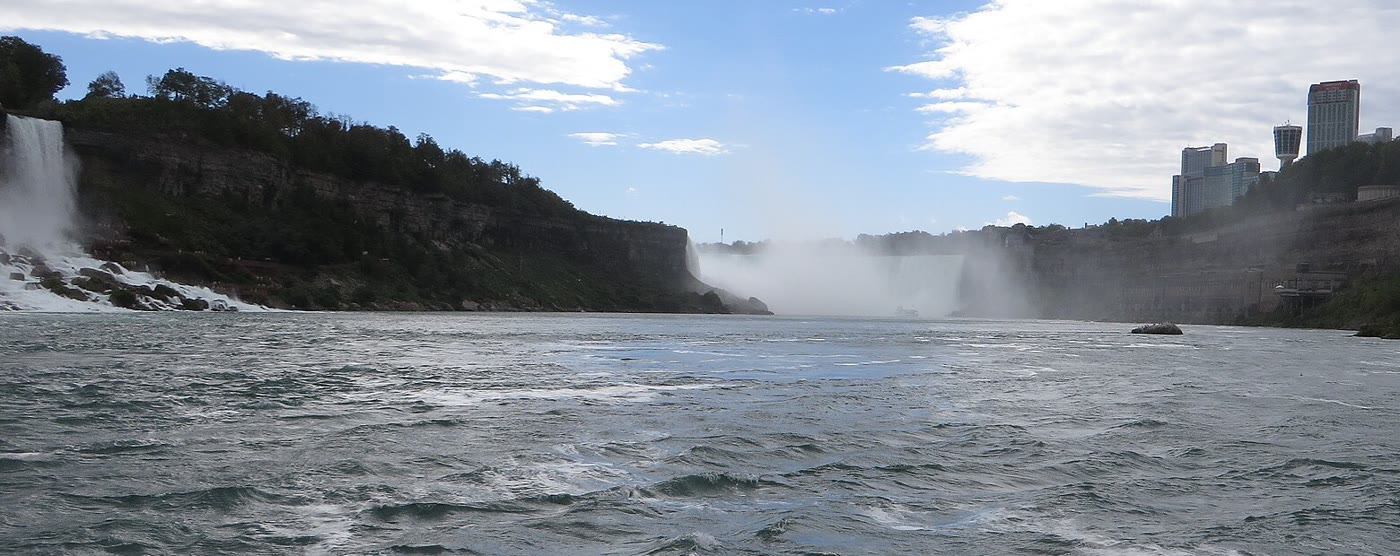
\includegraphics[width=\linewidth]{images/book5/b3-niagara-gorge.jpg}

{\scriptsize Het Niagararavijn, gezien stroomopwaarts naar de Hoefijzerwatervallen in
hun nevel, de Amerikaanse watervallen aan de linkerrand. Foto Ken Lund,
CC BY-SA 2.0 (bijgesneden).}
\end{minipage}
\end{inthefield}
% ledger: ijc18:niagara, photo:b3-niagara-gorge


\section{Glaciale erosie}\label{sec:b3:quantitative-geomorphology:glacial}

Een gletsjer die over zijn bed glijdt (basale glijding,
Hoofdstuk~\ref{ch:b3:glaciology}) erodeert het bed door schuring, waarbij puin dat in het
ijs zit het gesteente afschuurt, en door uitbraak, waarbij het blokken loswrikt die
door scheuren zijn losgemaakt. Beide schalen met de snelheid van de glijding.

\begin{definition}[Glaciale erosiewet]\label{def:b3:quantitative-geomorphology:glacial}
Een \emph{glaciale erosiewet}\index{glaciale erosiewet} geeft de erosiesnelheid van het bed van een
gletsjer als $E = K_G\,u_s^{\,l}$, waarin $u_s$ de
glijsnelheid is, $K_G$ een coëfficiënt en $l$ een exponent.
\end{definition}

Landschapsmodellen nemen meestal $l = 1$, waarbij waarden tussen 1 en 2 worden gebruikt.
Een compilatie van 38 gletsjers, waarvan de erosiesnelheden over vijf ordes van
grootte lopen, vond erosie gecorreleerd met de glijsnelheid, met $l = 0.65$ en
$K_G = 10^{-4}$ voor $E$ in meter per jaar: erosie is het snelst onder temperate
gletsjers die van ruime sneeuwval worden gevoed en die snel glijden. Omdat het ijs het dikst
en het snelst langs de as van een dal is, wordt de vloer dieper uitgesleten dan de zijkanten
en krijgt het dal zijn U-vorm.
% ledger: cook20:glacial

\begin{definition}[Glaciale cirkelzaag]\label{def:b3:quantitative-geomorphology:buzzsaw}
De \emph{glaciale cirkelzaag}\index{glaciale cirkelzaag} is de grens die gletsjers stellen aan de
hoogte van een bergketen: waar gesteente boven de hoogte uitsteekt waarop gletsjers ontstaan,
eroderen ze het net zo snel als het omhoog komt, ongeacht de opheffingssnelheid, zodat pieken en de
gemiddelde hoogte zich rond die hoogte concentreren.
\end{definition}

\section{Tektoniek en erosie}\label{sec:b3:quantitative-geomorphology:tectonics}

\begin{definition}[Topografische stationaire toestand]\label{def:b3:quantitative-geomorphology:steady-state}
Een landschap bevindt zich in een \emph{topografische stationaire toestand}\index{topografische stationaire toestand}
wanneer de erosiesnelheid overal gelijk is aan de opheffingssnelheid van het gesteente, zodat
de hoogten niet veranderen, hoewel er gesteente door het landschap heen beweegt.
\end{definition}

Snelheden die over verschillende tijdsduren zijn gemeten, toetsen de toestand. Kosmogene nucliden in
rivierzand geven de gemiddelde erosiesnelheid van een bekken over de tijd
die nodig is om een laag van de orde van de verzwakkingslengte van hun
productie weg te nemen, ongeveer \qty{55}{cm} gesteente; \omterm{def:b3:orogenic-wedges:thermochronology}{thermochronometers} en hun
\omterm{def:b3:orogenic-wedges:age-elevation}{ouderdom--hoogterelaties} geven de exhumatiesnelheid over miljoenen jaren. Waar de twee
onderling en met de opheffingssnelheid overeenkomen, bevindt het landschap zich waarschijnlijk
in \omterm{def:b3:quantitative-geomorphology:steady-profile}{stationaire toestand}; waar de kortetermijnsnelheid in de benedenloop sneller is dan in de bovenloop,
trekt er een \omterm{def:b3:quantitative-geomorphology:knickpoint}{knikpunt} door het gebied. Het wegnemen van gesteente ontlast ook de
lithosfeer, die daarop omhoog komt.
% ledger: zech04:exposure

\begin{definition}[Erosief isostatisch herstel]\label{def:b3:quantitative-geomorphology:rebound}
\emph{Erosief isostatisch herstel}\index{erosief isostatisch herstel} is
het oprijzen van het gesteenteoppervlak van een gebied in isostatisch evenwicht, als reactie op
de massa die door erosie is weggenomen.
\end{definition}

\begin{proposition}[Pieken rijzen terwijl dalen dieper worden]\label{prop:b3:quantitative-geomorphology:rebound}
In Airy-isostasie met korst van dichtheid $\rho_c$ over mantel van dichtheid
$\rho_m$, het wegnemen van een gemiddelde dikte $\bar e$ korst uit een gebied verhoogt
het hele gebied met $(\rho_c/\rho_m)\,\bar e$. Als de erosie beperkt blijft tot de dalen, rijzen de
niet-geërodeerde toppen met dat bedrag, terwijl het gemiddelde oppervlak slechts
met $(1 - \rho_c/\rho_m)\,\bar e$ daalt.
\end{proposition}

\begin{proof}
Compensatie vereist dat de massa van elke kolom boven een vaste diepte
gelijk blijft. Het wegnemen van een dikte $\bar e$ korst, gemiddeld over het
compensatiegebied, verlaagt de massa per oppervlakte-eenheid met $\rho_c \bar e$;
om die te vervangen moet mantel op diepte instromen, waardoor de basis van de
kolom, en alles erop, met $\delta$ opgetild, waarbij $\rho_m \delta = \rho_c \bar
e$. Een top die geen gesteente verloor, rijst met $\delta$; het gemiddelde oppervlak verliest
$\bar e$ en wint $\delta$.
\end{proof}

De gewogen dichtheid van de korst van het referentiemodel van de aarde is
\qty{2.72}{g/cm^3} en die van de mantel onder de Moho \qty{3.38}{g/cm^3},
een verhouding van 0.80: van elke honderd meter weggeërodeerd gesteente daalt het gemiddelde
oppervlak slechts twintig. Diepe insnijding van een oud plateau kan dus de toppen
doen rijzen, ook terwijl het plateau afslijt.
% ledger: prem:crust-mantle-ratio

\begin{omfigure}
\begin{tikzpicture}[x=0.6cm, y=0.6cm, font=\scriptsize]
\begin{scope}
\fill[omDef!12] (0,0) rectangle (8,4);
\draw[thick] (0,4) -- (8,4);
\draw[densely dashed] (0,0) -- (8,0);
\node[anchor=north] at (4,-0.1) {basis van de korst};
\node at (4,2) {korst $\rho_c$};
\node at (4,-1.2) {mantel $\rho_m$};
\node[anchor=south] at (4,4.1) {voor};
\end{scope}
\begin{scope}[xshift=6.2cm]
\fill[omDef!12] (0,0.8) -- (0,4.8) -- (1.4,4.8) -- (2.0,2.4) -- (2.6,4.8) -- (5.4,4.8) -- (6.0,2.4) -- (6.6,4.8) -- (8,4.8) -- (8,0.8) -- cycle;
\draw[thick] (0,4.8) -- (1.4,4.8) -- (2.0,2.4) -- (2.6,4.8) -- (5.4,4.8) -- (6.0,2.4) -- (6.6,4.8) -- (8,4.8);
\draw[black!50, densely dashed] (0,4) -- (8,4);
\draw[densely dashed] (0,0.8) -- (8,0.8);
\draw[densely dashed, black!40] (0,0) -- (8,0);
\draw[<->, omThm] (8.3,4.05) -- (8.3,4.75) node[midway, right] {$\delta$};
\draw[<->, omThm] (8.3,0.05) -- (8.3,0.75) node[midway, right] {$\delta$};
\node[anchor=west, font=\scriptsize] at (8.1,2.4) {$\delta = (\rho_c/\rho_m)\,\bar e$};
\node[anchor=south] at (4,5.0) {na insnijding van de dalen};
\node[anchor=north] at (2.0,2.3) {dal};
\end{scope}
\end{tikzpicture}

\par\smallskip{\small \omterm{def:b3:quantitative-geomorphology:rebound}{Erosief isostatisch herstel}, schematisch. Het uitsnijden
van de dalen verwijdert een gemiddelde dikte $\bar e$ aan korst; de kolom stijgt met
$\delta = (\rho_c/\rho_m)\bar e$ aan haar basis en op haar onaangeroerde toppen
(de grijze gestreepte lijn is het oude oppervlak).}\label{fig:b3:quantitative-geomorphology:rebound}
\end{omfigure}

\section{Oefeningen}

\begin{exercise}[$\star$]\label{exo:b3:quantitative-geomorphology:1}
Een kustescarpement met een verschuiving van \qty{4}{m} ($a = \qty{2}{m}$) ligt op een
hellingvlak op grote afstand met een helling van 0.04, en zijn steilste gradiënt is nu 0.30. Bereken
$\kappa t$, en daarna de ouderdom van het escarpement met $\kappa = \qty{5e-3}{m^2/yr}$.
\end{exercise}
% ledger: whipple04:scarp-erf, whipple04:scarp-kappa

\begin{exercise}[$\star$]\label{exo:b3:quantitative-geomorphology:2}
Een lidarmeting geeft een kromming van de heuvelkruin van \qty{-0.012}{m^{-1}} op een
rug met diffusiviteit \qty{4e-3}{m^2/yr}. Bereken de erosiesnelheid ervan in
\unit{mm/yr}, en het reliëf tussen de kam en de geulen
\qty{80}{m} verderop, uitgaande van een \omterm{def:b3:quantitative-geomorphology:steady-profile}{stationaire toestand}.
\end{exercise}

\begin{exercise}[$\star$]\label{exo:b3:quantitative-geomorphology:3}
Met $m = 0.5$, $n = 1$ en $K = \qty{2e-6}{yr^{-1}}$, bereken de
insnijsnelheid van een rivier die \qty{25}{km^2} afwatert op een gradiënt van 0.01.
Wat zijn de eenheden van $K$ voor algemene $m$ en $n$?
\end{exercise}

\begin{exercise}[$\star$]\label{exo:b3:quantitative-geomorphology:4}
Drie rivieren vertonen \omterm{def:b3:quantitative-geomorphology:knickpoint}{knikpunten}: (a) waar een zandsteenlaag een dal kruist dat
in schalie is uitgesneden; (b) waar een rivier een actieve afschuiving kruist van de
liggende naar de hangende wand; (c) in elke rivier van een bekken, allemaal op
ongeveer dezelfde hoogte, een paar kilometer boven een kust die bij een
aardbeving is opgeheven. Welke zijn vastgelegd en welke zullen migreren?
\end{exercise}

\begin{exercise}[$\star\star$]\label{exo:b3:quantitative-geomorphology:5}
Voor $m = 1$ en $n = 2$, bereken $\theta$ en de stationaire gradiënt waar $A =
\qty{10}{km^2}$, met $U = \qty{0.1}{mm/yr}$ en $K = 10^{-9}$ in meter en
jaar.
Met welke factor verandert de steilheid als $U$ verdubbelt? Vergelijk met $n =
1$.
\end{exercise}

\begin{exercise}[$\star\star$]\label{exo:b3:quantitative-geomorphology:6}
De afwateringsoppervlakte van een rivier groeit met de afstand $d$ tot haar waterscheiding als $A =
c\,d^{h}$. Toon aan dat, gemeten stroomopwaarts vanaf haar monding bij $d = L$,
\[
\chi(d) = \frac{A_0^{\theta}}{c^{\theta}}\,\frac{L^{p} - d^{p}}{p},
\qquad p = 1 - h\theta ,
\]
en bereken het voor $c = 2$ (SI), $h = 1.8$, $\theta = 0.45$, $A_0 =
\qty{1}{km^2}$, $L = \qty{20}{km}$ en $d = \qty{5}{km}$.
\end{exercise}

\begin{exercise}[$\star\star$]\label{exo:b3:quantitative-geomorphology:7}
Met $n = 1$, $m = 0.5$ en $K = \qty{2e-6}{yr^{-1}}$, bereken de
voortplantingssnelheid van een \omterm{def:b3:quantitative-geomorphology:knickpoint}{knikpunt} waar $A = \qty{100}{km^2}$, in m/kyr, en de
tijd die het zou kosten om \qty{5}{km} met die snelheid af te leggen. Waarom duurt
het in werkelijkheid langer?
\end{exercise}

\begin{exercise}[$\star\star$]\label{exo:b3:quantitative-geomorphology:8}
Dalen van \qty{600}{m} diep, die gemiddeld \qty{40}{\percent} van de
oppervlakte van een plateau innemen, worden erin uitgesneden. Met $\rho_c/\rho_m = 0.80$, bereken
de gemiddelde afgevoerde dikte, de stijging van de toppen en de verandering van de
gemiddelde hoogte.
\end{exercise}
% ledger: prem:crust-mantle-ratio

\begin{exercise}[$\star\star$]\label{exo:b3:quantitative-geomorphology:9}
Een \omterm{def:b3:quantitative-geomorphology:soil-production}{bodemproductiefunctie} heeft $P_0 = \qty{0.3}{mm/yr}$ en $h_0 =
\qty{0.5}{m}$. Bereken de stationaire bodemdikte bij erosie van
\qty{0.05}{mm/yr} en bij \qty{0.2}{mm/yr}. Wat gebeurt er bij
\qty{0.4}{mm/yr}?
\end{exercise}

\begin{exercise}[$\star\star\star$]\label{exo:b3:quantitative-geomorphology:10}
Een heuvel in \omterm{def:b3:quantitative-geomorphology:steady-profile}{stationaire toestand} erodeert met $E = \qty{0.1}{mm/yr}$ en $\kappa =
\qty{5e-3}{m^2/yr}$ en de niet-lineaire wet van de kritische gradiënt, waarbij
$S_c = 1.2$ voor de oefening wordt genomen. Toon aan dat de flux op afstand $x$ van de
waterscheiding gelijk is aan $E x$, los de gradiënt op en bereken die bij 20, 50, 100 en
\qty{200}{m}. Vergelijk met lineaire diffusie en beschrijf de
vorm van de heuvel.
\end{exercise}

\begin{exercise}[$\star\star\star$]\label{exo:b3:quantitative-geomorphology:11}
Toon aan dat de responstijd van een riviernetwerk op een verandering bij zijn monding,
voor $n = 1$, gelijk is aan $\chi_h/(K A_0^m)$, waarbij $\chi_h$ de grootste waarde van
$\chi$ bij een geulkop. Bereken die voor de bovenloop van de figuren
($A_0 = \qty{1}{km^2}$, $m = 0.5$, $K = \qty{e-6}{yr^{-1}}$), eerst voor de hoofdstam
alleen, waarvan de kop bij $\chi = \qty{5464}{m}$ ligt, daarna voor het netwerk,
waarvan de hoogste kop op zijrivier 1 bij $\chi = \qty{7237}{m}$ ligt.
\end{exercise}

\begin{exercise}[$\star\star\star$]\label{exo:b3:quantitative-geomorphology:12}
In een netwerk met $n = 1$ en uniforme $U$ stroomt één zijrivier over gesteente dat
twee keer zo erodeerbaar is als de rest ($2K$) boven haar samenvloeiing, bij $\chi_j$. Toon aan dat
haar stationaire lijn in het $(\chi, z)$-vlak heeft de helft van de helling van de
hoofdstam boven $\chi_j$, en dat een \omterm{def:b3:quantitative-geomorphology:knickpoint}{knikpunt} dat bij de monding ontstaat, bereikt
op het moment dat het \omterm{def:b3:quantitative-geomorphology:knickpoint}{knikpunt} van de hoofdstam bij $\chi_k > \chi_j$ ligt, het punt
van $\chi = \chi_j + 2(\chi_k - \chi_j)$ van die zijrivier.
\end{exercise}

\section{Probleem: De waterval van de Varden-rivier}

\begin{problem}[{Weekendprobleem --- het profiel, de steilheid en de erodeerbaarheid
van een verzonnen bovenloop, en de ouderdom van de waterval}]
\label{pb:b3:quantitative-geomorphology:1}
Ten westen van de Varden-heuvels stroomt de rivier door een hooggelegen gebied van
schist voordat ze de kaart aan haar westrand binnenkomt, op een hoogte van \qty{170}{m}. Stroomopwaarts
van dat punt, haar monding, is de hoofdstam \qty{12}{km} lang vanaf haar
waterscheiding, met een afwateringsoppervlakte $A = 4.5\,d^{1.7}$ (\unit{m^2}, $d$ in meter vanaf de
waterscheiding) en een geulkop bij $d = \qty{300}{m}$. Neem als de snelheid van de
gesteenteopheffing de denudatiesnelheid van het bekken van de Varden-rivier, gevonden uit
haar vrachten in Boek~3, \qty{43}{m/Myr}. Neem $n = 1$ en het referentiegebied $A_0 = \qty{1}{km^2}$.
Een waterval van \qty{25}{m} hoog staat op de hoofdstam \qty{4.60}{km} stroomopwaarts van de
monding. Alle waarden zijn verzonnen.

\medskip\noindent\textbf{Part I --- The profile.}
\begin{enumerate}
\item Bereken de afwateringsoppervlakte aan de monding en aan de geulkop.
\item Gradiënten gemeten over trajecten van \qty{200}{m}, weg van de
  waterval:

  \smallskip
  {\small\begin{tabular}{l*{6}{c}}
  $A$ (\unit{km^2}) & 0.388 & 0.587 & 0.888 & 1.345 & 2.036 & 3.082 \\
  $S$ & 0.06641 & 0.05026 & 0.04888 & 0.03322 & 0.03688 & 0.02688 \\[2pt]
  $A$ (\unit{km^2}) & 4.665 & 7.061 & 10.69 & 16.18 & 24.49 & 37.08 \\
  $S$ & 0.01921 & 0.01713 & 0.01545 & 0.01419 & 0.007922 & 0.007855
  \end{tabular}}

  \smallskip
  Schat de \omterm{def:b3:quantitative-geomorphology:indices}{concaviteitsindex} uit het eerste en het laatste punt.
\item De kleinste-kwadratenhelling van $\log S$ tegen $\log A$ is $-0.466$.
  Is dit in overeenstemming met $\theta = 0.5$?
\item Bereken met $\theta_{\mathrm{ref}} = 0.5$ de waarde $k_{sn} = S A^{0.5}$ ($A$ in
  \unit{m^2}) voor het eerste en het laatste punt, en geef aan wat het
  geometrische gemiddelde van de twaalf waarden, \qty{45.1}{m}, voorstelt.
\item Waarom variëren de gradiënten veel sterker dan de hoogten?
\item Bereken met de formule van de chi-oefening $\chi$ op $d =
  \qty{9.00}{km}$, een punt onder de waterval.
\end{enumerate}

\medskip\noindent\textbf{Deel II --- Steilheid en erodeerbaarheid.}
\begin{enumerate}[resume]
\item De rivier ligt op \qty{193.4}{m} bij $d = \qty{9.00}{km}$. Bereken de
  helling van de chi-plot onder de waterval en de steilheid $k_{sn}$.
\item Welke schatting van $k_{sn}$ zou je vertrouwen, deze of die uit de
  helling-oppervlakte-methode, en waarom?
\item Bereken, uitgaande van een \omterm{def:b3:quantitative-geomorphology:steady-profile}{stationaire toestand} onder de waterval, $K$
  uit de opheffingssnelheid.
\item Controleer dat de insnijdingssnelheid aan de monding, waarvan de helling
  0.00691 is, gelijk is aan de opheffingssnelheid.
\item Bereken de snelheid van een \omterm{def:b3:quantitative-geomorphology:knickpoint}{knikpunt} aan de monding en bij de waterval,
  in m/kyr.
\item Bereken de hoogte van de geulkop op het stationaire profiel, en het
  reliëf van de hoofdstam.
\end{enumerate}

\medskip\noindent\textbf{Deel III --- De waterval.}
\begin{enumerate}[resume]
\item Waarom heeft de waterval, met $n = 1$, de hoogte van de val van het
  \omterm{def:b3:quantitative-geomorphology:knickpoint}{basisniveau} behouden?
\item Bereken $\chi$ bij de waterval.
\item Bereken de tijd die het \omterm{def:b3:quantitative-geomorphology:knickpoint}{knikpunt} nodig had van de monding tot zijn
  huidige plaats.
\item Waar zal het \qty{300}{kyr} vanaf nu zijn?
\item Zijrivier 3 mondt \qty{2.5}{km} stroomopwaarts van de monding in de
  hoofdstam uit; ze is \qty{5}{km} lang, met $A = 1.5\,s^{1.7}$ ($s$ vanaf
  haar eigen waterscheiding). Waar zou haar waterval moeten liggen?
\item Zijrivieren 1 en 2 monden \qty{8}{km} en \qty{5}{km} stroomopwaarts van
  de monding in de hoofdstam uit. Verklaar waarom zij geen waterval hebben.
\end{enumerate}

\medskip\noindent\textbf{Deel IV --- De hellingen en de ouderdom.}
\begin{enumerate}[resume]
\item Een lidar-meting boven de waterval geeft een kromming van de heuveltop
  van \qty{-0.0086}{m^{-1}}. Bereken met $\kappa = \qty{5e-3}{m^2/yr}$ de
  erosiesnelheid en vergelijk die met de opheffingssnelheid.
\item De hellingen zijn ongeveer \qty{150}{m} lang. Vergelijk hun
  responstijd $L^2/\kappa$ met de ouderdom uit Deel III.
\item Beschrijf de hellingen onder de waterval zoals ze er nu uitzien, en hoe
  ze zullen veranderen.
\item De opheffingssnelheid is bekend tot op \qty{20}{\percent}. Geef het
  bereik van de ouderdom.
\item Hoe zou de waterval zich hebben ontwikkeld als $n$ gelijk was aan 2?
\item Geef de ouderdom van de val van het \omterm{def:b3:quantitative-geomorphology:knickpoint}{basisniveau}.
\end{enumerate}
\end{problem}
% ledger: whipple04:steepness, whipple04:scarp-kappa
